%   % !TEX root = ../../VIII,3_Rahmen-TeX_9-0.tex
%  
%   Band VIII, 3 N.~?? 	Stoß??			(Unter)rubrik			??
%   Signatur/Tex-Datei:	LH_37_05_016
%   RK-Nr. 	57272
%				
%   Überschrift: 	(keine)
%   Titel: 			??			(unser Titel)					??
%   Datierung:		?? (Juni??) 1677 bis Jan 1678???? (a. St.)
%   Textfolge: 					wie Foliierung
%   WZ: 	Blattrand, Nr. 803005 (Fragment)							??
%   edlabels:			3
%   Diagramme: 		1
%   Dateien (PDF):
%   		LH_37_05_016-d_016r
%
%   Erstaufnahme:			(wer?)
%   Bearbeitung MS ab: 		August 2020
%
%   NB: 						(Anmerkungen)					??
%
%
\selectlanguage{ngerman}
\frenchspacing
%
\begin{ledgroupsized}[r]{120mm}
\footnotesize
\pstart
\noindent\textbf{Überlieferung:}
\pend
\end{ledgroupsized}
%
\begin{ledgroupsized}[r]{114mm}
\footnotesize
\pstart \parindent -6mm
\makebox[6mm][l]{\textit{L}}%
Konzept:
LH~XXXVII~5~Bl.~16.
Ein Blatt~4\textsuperscript{o};
Wasserzeichenfragment am Blattrand;
Papiererhaltungsmaßnahmen;
alle Ränder beschnitten.
Zwei Seiten.
\pend
\end{ledgroupsized}
%
\begin{ledgroupsized}[r]{114mm}
\footnotesize
\pstart
\parindent -6mm
\makebox[6mm][l]{\textit{E}}%
(tlw.) \cite{01056}\textsc{Fichant} 1994, S.~387f.
\pend%
\end{ledgroupsized}
%
%
\vspace{5mm}
\begin{ledgroup}
\footnotesize
\pstart
\noindent%
\textbf{Datierungsgründe:} %%
Im vorliegenden Konzept führt Leibniz die Analyse eines einfachen Stoßfalls auf der Grundlage der in anderen Stücken erörterten 
%
(\glqq alibi explicata\grqq) Schiffsanalogie durch.
%
Hinter den scheinbar erfolgreichen Berechnungen dieser Methode (\glqq haec quidem optime procedunt in speciem\grqq)
%
verbirgt sich eine \glqq difficultas ingens\grqq, weil die Erhaltung der \textit{vis}  oder \textit{potentia},
%
hier als die skalare Größe $mv$ aufgefasst, nicht gewährleistet ist.
%
\pend
%
\pstart
Aufschluss über die Entstehungszeit von N.~\ref{RK57272} geben zunächst Leibnizens Anspielungen auf seine Ausführungen in anderen Stücken (\glqq alibi\grqq)
%
bezüglich der Schiffsanalogie und der Verformung elastischer Körper beim Stoß.
%
Die Anspielungen gelten höchstwahrscheinlich den Konzepten N.~\ref{RK57269} und N.~\ref{RK57271} vom 10.\ und 11.\ (20.\ und 21.) Juni 1677.
%
Die ausdrückliche Gleichsetzung der Kraft mit der Bewegungsgröße auf S.~\refpassage{37_05_016_3a}{37_05_016_3b} (\glqq Nam si celeritates in pondera ducantur habebimus vim\grqq)
%
deutet auf die Entstehung von N.~\ref{RK57272} vor der Annahme des quadratischen Kraftmaßes,
%
also vor \textit{De corporum concursu}, \textit{Scheda octava} von Januar 1678 (N.~\ref{dcc_08}), hin.
%
Daraus ergibt sich für N.~\ref{RK57272} die Datierungsspanne Ende Juni 1677 bis Januar 1678.
%
Auch für die Konzepte N.~\ref{RK57276} und N.~\ref{RK57275} wird dieselbe Zeitspanne ermittelt; 
%
dabei kann festgestellt werden, dass 
%
während in letzteren Stücken das Problem der Nichterhaltung der Bewegungsgröße beim Stoß
%
im Laufe der Berechnungen und gleichsam wider Erwarten auftritt,
%
das vorliegende Konzept strukturierter verfährt, d.\,h.\ nach einer Vorführung der Vorzüge der Schiffsanalyse
%
ebenjene \glqq difficultas ingens\grqq\ ankündigt und sie anhand gut gewählter numerischer Werte darlegt.
%
Dieser Umstand lässt die Vermutung zu, dass Leibniz mit N.~\ref{RK57272} eine methodisch konstruierte Darstellung
%
der Schwierigkeiten, die er zuvor in N.~\ref{RK57276} und N.~\ref{RK57275} festgestellt hatte, bieten wollte
%
\textendash\ und demnach N.~\ref{RK57272} nach den beiden anderen Stücken verfasst haben könnte.
\pend
%
%%
\end{ledgroup}
%
%\newpage%
%
\selectlanguage{latin}
\frenchspacing
\vspace{8mm}
\pstart%
\normalsize%
\noindent%
\lbrack16~r\textsuperscript{o}\rbrack\
%
%
%
%
Duo globi\protect\index{Sachverzeichnis}{globus}
%
\edtext{volumine aequales\protect\index{Sachverzeichnis}{globi volumine aequales}}{\lemma{}\Bfootnote{volumine aequales \textit{erg.}~\textit{L}}}
%
\textit{M.N.} sint in ratione 
%
\edtext{ponderis}{\lemma{}\Bfootnote{ponderis \textit{erg.}~\textit{L}}}
%
dupla, seu
%
\textit{M} aequ.
%
\edtext{2\textit{N}\lbrack,\rbrack\ ambo collocat\lbrack i\rbrack}{\lemma{2\textit{N}}\Bfootnote{\textit{(1)}~in m \textit{(2)}~erit cor \textit{(3)}~ambo \textbar\ collocata \textit{ändert Hrsg.} \textbar\ in~\textit{L}}}
%
in extremis rectae \textit{AB.}, nempe \textit{M} in \textit{A} et \textit{N} in \textit{B}.
%
Eorum centrum gravitatis\protect\index{Sachverzeichnis}{centrum gravitatis} erit \textit{C}, posito
%
\textit{AC} aequ.\ $\displaystyle\frac{1}{3}AB$.
%
\rule[0cm]{0mm}{16pt}%
Ponantur sibi directe occurrere in eadem recta \textit{AB}, erit punctum concursus \protect\index{Sachverzeichnis}{punctum concursus} \textit{D}, 
%
\rule[0cm]{0mm}{10pt}\edtext{medium rectae}{\lemma{medium}\Bfootnote{\textbar\ scilicet \textit{gestr.}\ \textbar\ rectae~\textit{L}}}
%
\textit{AB}.
%
\edtext{Quod si jam secundum alibi explicata fingamus, concursum\protect\index{Sachverzeichnis}{concursus} hunc ita explicari, ut perinde sit ac si ferantur in navi\protect\index{Sachverzeichnis}{navis}}{\lemma{Quod \lbrack...\rbrack\ in navi}\Cfootnote{Siehe die ausführliche Behandlung des Stoßes anhand der  Schiffsanalogie in N.~\ref{RK57269} vom 10.\ (20.) Juni 1677.}}
%
quae feratur 
\pend
%
\newpage
\vspace{1.0em} %%%%%%%%% Diagramm 1
\centerline{%
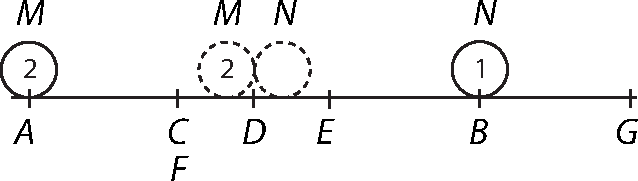
\includegraphics[width=0.48\textwidth]{%
gesamttex/edit_VIII,3/images/LH_37_05_016_d_016r.pdf%
}} 
\vspace{0.2em}
\centerline{%
\lbrack\textit{Fig.~1}\rbrack%
}
\vspace{1em}
%\newpage%
\pstart\noindent
celeritate
\textit{CD}.\ ita ut \textit{M} feratur celeritate \textit{AC} et \textit{N} celeritate
%
\edtext{\textit{BC}., tunc celeritate \textit{CD}}{\lemma{\textit{BC}.,}\Bfootnote{\textit{(1)}~et centro \textit{(a)}~celerit \textit{(b)}~gravitatis seu navi porro progrediente ex \textit{D} in \textit{E}, \textit{(2)}~tunc \textbar\ celeritate \textit{erg.}\ \textbar\ \textit{CD}~\textit{L}}}
%
appellata \textit{x}
feretur corpus \textit{M} 
%
\edtext{celeritate ut \textit{AC} seu 2\textit{x}.}{\lemma{celeritate}\Bfootnote{\textit{(1)}~3\textit{x} \textit{(2)}~ut \textit{AC} seu 2\textit{x}.~\textit{L}}}
%
et corpus \textit{N} celeritate ut \textit{BC} seu 4\textit{x}\lbrack,\rbrack\
%
quae cum sit ipsis corporibus reciproca,\protect\index{Sachverzeichnis}{celeritates reciprocae corporibus}
%
utique aequali vi concurrent, adeoque
%
ea quae venere celeritate repercutientur. Nam navi\protect\index{Sachverzeichnis}{navis} seu centro gravitatis\protect\index{Sachverzeichnis}{centrum gravitatis}
%
progrediente in \textit{E}, interim corpus 
%
\edtext{\textit{M} regredietur}{\lemma{\textit{M}}\Bfootnote{\textit{(1)}~ex \textit{D} \textit{(2)}~regredietur ~\textit{L}}}
%
ex \textit{E} celeritate
%
\edtext{\textit{EF}}{\lemma{\textit{EF}}\Bfootnote{\textit{erg.}~\textit{L}}}
%
quae sit aequalis ipsi
%
\edtext{\textit{AC}, sed haec}{\lemma{\textit{AC},}\Bfootnote{\textit{(1)}~quae \textit{(2)}~sed haec~\textit{L}}}
%
ab \textit{A} retro sumta est \textit{EC}, ergo hoc loco
coincidunt
%
\edtext{\lbrack\textit{C}\rbrack}{%
\lemma{}%
\Bfootnote{%
\textit{E} %
\textit{L ändert Hrsg.}%
}}
%
et \textit{F}, at corpus \textit{N} 
%
\edtext{ab \textit{E} repelletur}{%
\lemma{ab \textit{E}}%
\Bfootnote{%
\textit{(1)}~repellitur %
\textit{(2)}~repelletur~\textit{L}%
}}
%
celeritate aequali ipsi 
%
\edtext{\lbrack\textit{BC}\rbrack,}{%
\lemma{\textit{EC}}%
\Bfootnote{%
\textit{L ändert Hrsg.}}}
%
adeoque ea erit \textit{EG}, et ita hoc loco erit \textit{BG} aequ.\ \textit{EB}. 
\pend 
%
\pstart
Haec quidem optime procedunt in speciem; sed intus latet difficultas ingens.\protect\index{Sachverzeichnis}{difficultas ingens}
%
\edlabel{37_05_016_3a}Nam si celeritates in pondera ducantur\protect\index{Sachverzeichnis}{celeritas in pondus ducta} habebimus
%
vim;\protect\index{Sachverzeichnis}{vis}\edlabel{37_05_016_3b}
%
vis\protect\index{Sachverzeichnis}{vis} autem seu
potentia\protect\index{Sachverzeichnis}{potentia} nec crescere nec minui potest. Quorum tamen alterutrum hoc
loco contingit.%
\pend
%
\pstart
Nempe corpus \textit{M} aequ.\ 
%
\edtext{2\textit{N}. Et revera}{\lemma{2\textit{N}.}\Bfootnote{\textit{(1)}~Ergo et celeritas ejus \textit{EC} aequ.\ 2\textit{x} \textit{(2)}~Et revera~\textit{L}}}
%
reperitur hoc modo regressum esse a \textit{D} in \textit{F}
ergo 
%
%
\edlabel{37_05_016_1a}%
\edtext{}{% C-Footnote – x und (x)
{\xxref%
{37_05_016_1a}{37_05_016_1b}}%
\lemma{ejus celeritas \lbrack...\rbrack\ $\dfrac{9}{7}x$}%
\Cfootnote{%
In der Passage auf S.~\refpassage{37_05_016_1a}{37_05_016_2} bezeichnet Leibniz die Geschwindigkeitseinheit vor und nach dem Stoß jeweils mit \textit{x} und (\textit{x}), hält jedoch diese Regel im nachfolgenden Absatz nicht mehr konsequent ein.%
}}%
ejus celeritas est
%
\edtext{1(\textit{x}). Ergo}{%
\lemma{}%
\Bfootnote{%
1(\textit{x}). \textbar\ Quia ita \textit{erg., streicht Hrsg.}~\textbar\ Ergo~\textit{L}%
}}
%
vis ejus $2N(x)$.
%
Corpus autem \textit{N} aequ.\ \textit{N}.\
et celeritas ejus \textit{DG}, aequ.\ $5(x)$.
%
Ergo vis ejus aequ.\ $5N(x)$, summa ergo 
virium $2N(x) + 5N(x)$ aequ.\ $7N(x)$. At qualis ante concursum\protect\index{Sachverzeichnis}{concursus} fuerit sic apparet\lbrack:\rbrack\
%
 \textit{AD} aequ.\ 
%
\edtext{\textit{BD} aequ.\ 3\textit{CD}.}{%
\lemma{\textit{BD} aequ.}%
\Bfootnote{%
\textit{(1)}~3\textit{x} %
\textit{(2)}~3\textit{CD}.~\textit{L}%
}}
%
ergo celeritas concursus\protect\index{Sachverzeichnis}{celeritas concursus} utrobique 
aequalis erit 3\textit{x}, ducta in corpus\protect\index{Sachverzeichnis}{celeritas ducta in corpus} \textit{M} seu 2\textit{N} dat 6\textit{Nx}. 
%
Ducta in corpus\protect\index{Sachverzeichnis}{celeritas ducta in corpus}
%
\edtext{\textit{N} dat}{%
\lemma{}%
\Bfootnote{%
\textit{N} \textbar\ seu \textit{streicht Hrsg.}\ \textbar\ %
dat~\textit{L}}}
%
3\textit{Nx}, summa virium\protect\index{Sachverzeichnis}{summa virium} est 9\textit{Nx}. Supra erat 
%
\edtext{$7N(x)$. Ergo}{\lemma{$7N(x)$}\Bfootnote{\textit{(1)}~, \textbar~pro \textit{streicht Hrsg.}\ \textbar\ %
\textit{x} \textbar\ in posteriori \textit{erg.}\ \textbar\ 
scribamus \textit{y}, fiet 9\textit{Nx} aequ.\ 7\textit{Ny} seu \textit{(2)}~. Ergo~\textit{L}}}
%
$(x)$ aequ.\ $\displaystyle\frac{9x}{7}$.
%
\rule[0cm]{0mm}{16pt}%
Ita enim
%
$\displaystyle\frac{18}{7}x+\displaystyle\frac{45}{7}x$ aequ.\ $\displaystyle\frac{63}{7}x$ aequ.\ 9\textit{x}.%
\edlabel{37_05_016_2}%	%zwecks Referenzierung
%
\pend
%
\pstart
%
\rule[0cm]{0mm}{10pt}%
Videamus an idem prodeat, si statim ab initio instituamus aequationem, nempe quando fingitur corpus \textit{M} moveri celeritate
%
\edtext{\textit{AC}, et}{\lemma{}\Bfootnote{\textit{AC}, \textbar~seu \textit{erg., streicht Hrsg.}\ \textbar\ et~\textit{L}}}
%
corpus 
%
\edtext{\lbrack\textit{N}\rbrack}{%
\lemma{}%
\Bfootnote{%
\textit{M} %
\textit{L ändert Hrsg.}%
}}
%
celeritate 
\textit{BC}, tunc vis corporis 
%
\edtext{\textit{M} est 2\textit{N}}{%
\lemma{\textit{M} est}%
\Bfootnote{%
\textit{(1)}~4\textit{x} %
\textit{(2)}~2\textit{N}~\textit{L}%
}}
%
in $2(x)$ seu $4N(x)$. Vis\protect\index{Sachverzeichnis}{vis} corporis 
%
\edtext{\lbrack\textit{N}\rbrack}{%
\lemma{}%
\Bfootnote{%
\textit{N} %
\textit{erg. Hrsg.}%
}}
%
est $4N(x)$
seu utraque vis\protect\index{Sachverzeichnis}{vis} est aequalis. Fit summa harum duarum $8N(x)$, quibus si addatur 
vis competens toti navi\protect\index{Sachverzeichnis}{vis competens navi}\protect\index{Sachverzeichnis}{navis} (a cujus vi abstrahemus) ob motum
%
\edtext{communem\protect\index{Sachverzeichnis}{motus communis} per \textit{CD}}{\lemma{communem}\Bfootnote{\textit{(1)}~\textit{CD}, fiet vis \textit{(2)}~per \textit{x} \textit{(3)}~per \textit{CD}~\textit{L}}},
%
seu $1(x)$ summae corporum 2\textit{N} et 1\textit{N} seu 3\textit{N}, fiet
vis\protect\index{Sachverzeichnis}{vis} hinc orta $3N(x)$, quae priori 8\textit{Nx} addita dat $11N(x)$, cum debeat esse
tantum 9\textit{Nx}. 
%
\rule[0cm]{0mm}{16pt}%
Ergo $(x)$ aequ.\ $\displaystyle\frac{11}{9}x$, non vero ut ante $\displaystyle\frac{9}{7}x$.%
\edlabel{37_05_016_1b}
%
%
Ergo ictus\protect\index{Sachverzeichnis}{ictus} 
%%%%%%%%%%%%%%%%%%%%%%%
%%
%%      End of 16r
%%
%%%%%%%%%%%%%%%%%%%%%%%
%%
%%   Fol. 16v.
%%
%%%%%%%%%%%%%%%%%%%%%%%%
%
\lbrack16~v\textsuperscript{o}\rbrack\
%
\rule[0cm]{0mm}{10pt}%
a corporibus exceptus erit 
%
$\displaystyle\frac{72}{7}x$.\
%
et 
%
\edtext{in singulo}{%
\lemma{in}%
\Bfootnote{%
\textit{(1)}~singula %
\textit{(2)}~singulo~\textit{L}%
}}
%
eorum recipietur
vis
%
\rule[0cm]{0mm}{16pt}%
$\displaystyle\frac{36x}{7}$.
%
Quoniam autem hoc modo etiam ambo corpora 
\rule[0cm]{0mm}{10pt}%
repercutientur,
ideo corpus \textit{M} progrediens celeritate \textit{x} et vi 2\textit{x}, regrediens 
vero vi 
%
$\displaystyle\frac{36}{7}x$,
%
debebit omnino regredi
%
\edtext{nam restabit}{\lemma{}\Bfootnote{nam \textbar\ nam \textit{streicht}\ \textit{Hrsg.}\ \textbar\ restabit~\textit{L}}} 
%
\rule[0cm]{0mm}{16pt}%
$\displaystyle\frac{22}{7}x$,
%
qua
regredietur. 
\rule[0cm]{0mm}{10pt}%
Quod omnino absurdum est, ita enim vincet debilius,\protect\index{Sachverzeichnis}{corpus debilius} saltem
fortius\protect\index{Sachverzeichnis}{corpus fortius} finem suum non assequetur.
%
\pend \pstart
%
Ictus\protect\index{Sachverzeichnis}{ictus} est aestimandus ex resistentia.\protect\index{Sachverzeichnis}{resistentia}
%
Oritur autem resistentia\protect\index{Sachverzeichnis}{resistentia} ex duobus capitibus,
primum ex vi\protect\index{Sachverzeichnis}{vis} corporis obnitentis\protect\index{Sachverzeichnis}{corpus obnitens} quae detrahenda est a vi\protect\index{Sachverzeichnis}{vis} procedentis\protect\index{Sachverzeichnis}{corpus procedens}; 
%
deinde ex eo, quod 
etsi corpus aliquod quiescat, seu nulla vi obnitatur, nihilominus celeritatem progredientis
%
\edtext{debilitat. Rem}{\lemma{debilitat.}\Bfootnote{\textit{(1)}~Sed rem vix \textit{(2)}~Rem~\textit{L}}}
%
succedere video in corporibus aequalibus,\protect\index{Sachverzeichnis}{corpora aequalia} ut si corpus
unum incurrat in aliud quiescens,\protect\index{Sachverzeichnis}{incursus corporis in aliud quiescens} utique si secum abripit dat ei dimidium sui impetum.\protect\index{Sachverzeichnis}{impetus}
%
Ergo et resistentia\protect\index{Sachverzeichnis}{resistentia} tanta erit. Ergo sic resistentia\protect\index{Sachverzeichnis}{resistentia} erit
%
\edtext{aequalis vi residuae.\protect\index{Sachverzeichnis}{vis residua} Ergo compressio\protect\index{Sachverzeichnis}{compressio}}{\lemma{aequalis}\Bfootnote{\textit{(1)}~ictui residuo. Fiet \textit{(2)}~vi residuae. Ergo
\textit{(a)}~tota \textit{(b)}~tensio \textit{(c)}~compressio~\textit{L}}}
%
corporum durorum\protect\index{Sachverzeichnis}{corpora dura} eadem erit, quae 
vis totius,\protect\index{Sachverzeichnis}{vis totius} sed hoc absurdum, quia hoc demum fit, cum
%
\edtext{aequali celeritate}{\lemma{aequali}\Bfootnote{\textit{(1)}~vi moventur. Er \textit{(2)}~celeritate~\textit{L}}}
%
corpora aequalia\protect\index{Sachverzeichnis}{corpora aequalia} concurrunt.
\pend \pstart
Vis\protect\index{Sachverzeichnis}{vis} semper eadem manet.
\pend \pstart
Si considerentur 
%
\edtext{quae alibi dixi, de corpore antea comprimente, 
%
\edtext{quam impellente,}{\lemma{quam}\Bfootnote{\textit{(1)}~imprimente \textit{(2)}~impellente,~\textit{L}}}%
}{\lemma{quae \lbrack...\rbrack\ impellente}%
\Cfootnote{Siehe S.~\refpassage{37_05_159-160_8a}{37_05_159-160_8b} von N.~\ref{RK57271}.}}
%
sequitur corpus in
%
\edtext{quiescens}{\lemma{}\Bfootnote{quiescens \textit{erg.}~\textit{L}}}
%
aequale et 
%
\edtext{simile impingens,\protect\index{Sachverzeichnis}{corpus in quiescens aequale impingens}}{\lemma{}\Bfootnote{simile \textbar\ et \textit{erg., streicht Hrsg.}\ \textbar\ impingens,~\textit{L}}}
%
diversimode agere
pro diversa vi ictus.\protect\index{Sachverzeichnis}{vis ictus} Si tarde moveatur,
%
\edtext{erit mox}{\lemma{erit}\Bfootnote{\textit{(1)}~statim \textit{(2)}~mox~\textit{L}}}
%
vis compressionis\protect\index{Sachverzeichnis}{vis compressionis} major vi residua\protect\index{Sachverzeichnis}{vis residua}
%
et corpus impressionem accipiens propelletur, alterum autem non repelletur, 
%
\edtext{si plus}{\lemma{si}\Bfootnote{\textit{(1)}~satis \textit{(2)}~plus~\textit{L}}}
%
ei 
%
\edtext{virium restat,}{\lemma{virium}\Bfootnote{\textit{(1)}~quam a repulsu \textit{(2)}~restat,~\textit{L}}}
%
quam a repulsu compressionis\protect\index{Sachverzeichnis}{compressio} retro accipit. Potest
et tanta celeritate moveri, 
%
\edtext{ut compressionis vis\protect\index{Sachverzeichnis}{vis compressionis}}{\lemma{ut}\Bfootnote{\textit{(1)}~compressio aequalis \textit{(2)}~compressionis vis~\textit{L}}}
%
dimidia fit aequalis vi residuae,\protect\index{Sachverzeichnis}{vis residua}
seu ut residua vis\protect\index{Sachverzeichnis}{vis residua} sit
%
\edtext{tertia pars}{\lemma{tertia}\Bfootnote{\textit{(1)}~vis totius \textit{(2)}~pars~\textit{L}}}
%
totius vis, et tunc quiescet
corpus impellens.\protect\index{Sachverzeichnis}{corpus impellens}
\pend 
%
\pstart
Imo sic, post compressionem\protect\index{Sachverzeichnis}{compressio} corpus impellens\protect\index{Sachverzeichnis}{corpus impellens}
pergit celeritate non quae ei restabat, sed minore ob corpus quod impellit.
Ex.~gr.\ si ei aequalis dimidiae 
%
\edtext{rest\lbrack et,\rbrack}{%
\lemma{restantis.}%
\Bfootnote{%
\textit{L ändert Hrsg.}%
}}
%
quae si etiam aequalis
sit dimidiae compressionis,\protect\index{Sachverzeichnis}{vis compressionis} tunc quiescit denique corpus impellens\protect\index{Sachverzeichnis}{corpus impellens}, et
tota vis transfertur\protect\index{Sachverzeichnis}{translatio totius vis} in 
%
\edtext{impulsum.\protect\index{Sachverzeichnis}{corpus impulsum} Imo}{\lemma{impulsum.}\Bfootnote{\textit{(1)}~Ergo quando \textit{(a)}~vis \textit{(b)}~vis compressionis tanta est ut vis ictus \textit{(2)}~Imo~\textit{L}}}
%
videtur 
%
\edtext{semper vis ictus}{\lemma{semper vis}\Bfootnote{\textit{(1)}~compressionis suf \textit{(2)}~ictus~\textit{L}}}
%
ad comprimendum sufficiens. Nam si magna est multum comprimit, si parva
parum; semper ergo videtur corpus comprimere, donec vis compressionis\protect\index{Sachverzeichnis}{vis compressionis} 
satis magna sit vel ad unum corpus repellendum, vel ad alterum 
propellendum. Et hinc videntur omnia determinari posse.
\pend \pstart
Nondum mihi satisfeci.
\pend
\count\Afootins=1200%
\count\Bfootins=1200%
\count\Cfootins=1200